\documentclass[tikz, border=25pt]{standalone}
\usepackage[utf8]{inputenc}
\usepackage[T5]{fontenc}
\usepackage{lmodern}
\usepackage{xcolor}
\usepackage{graphicx}
\usetikzlibrary{positioning, calc, arrows}

\begin{document}
\begin{tikzpicture}[
  >=stealth,
  font=\sffamily,
  % Card khung nét đứt to rõ, nền trắng tinh
  tierCard/.style={
    draw=black,
    dashed,
    line width=2.0pt,
    fill=white,
    rounded corners=8pt,
    inner sep=12pt,
    align=center
  },
  % Nhãn trên mũi tên chữ to đậm, viền rõ ràng
  tagText/.style={
    font=\fontsize{14}{17}\selectfont\bfseries,
    fill=white,
    inner sep=4.5pt,
    rounded corners=3pt,
    draw=black,
    line width=1.0pt,
    text=black
  },
  arrowThick/.style={
    ->,
    line width=2.8pt,
    draw=black
  },
  biArrowThick/.style={
    <->,
    line width=2.8pt,
    draw=black
  }
]

% ==================== 1. TẦNG 4: THỊ GIÁC 3D (ĐẶT Ở TRÊN CÙNG) ====================
\node[tierCard, text width=13.5cm] (tier4) at (0, 6.0) {
  {\fontsize{21}{25}\selectfont\bfseries TẦNG 4: THỊ GIÁC 3D \& TÁC VỤ}\\[3pt]
  {\fontsize{13}{16}\selectfont\color{black!75} (Vision Pre-Actuation Tier)}\\[8pt]
  
  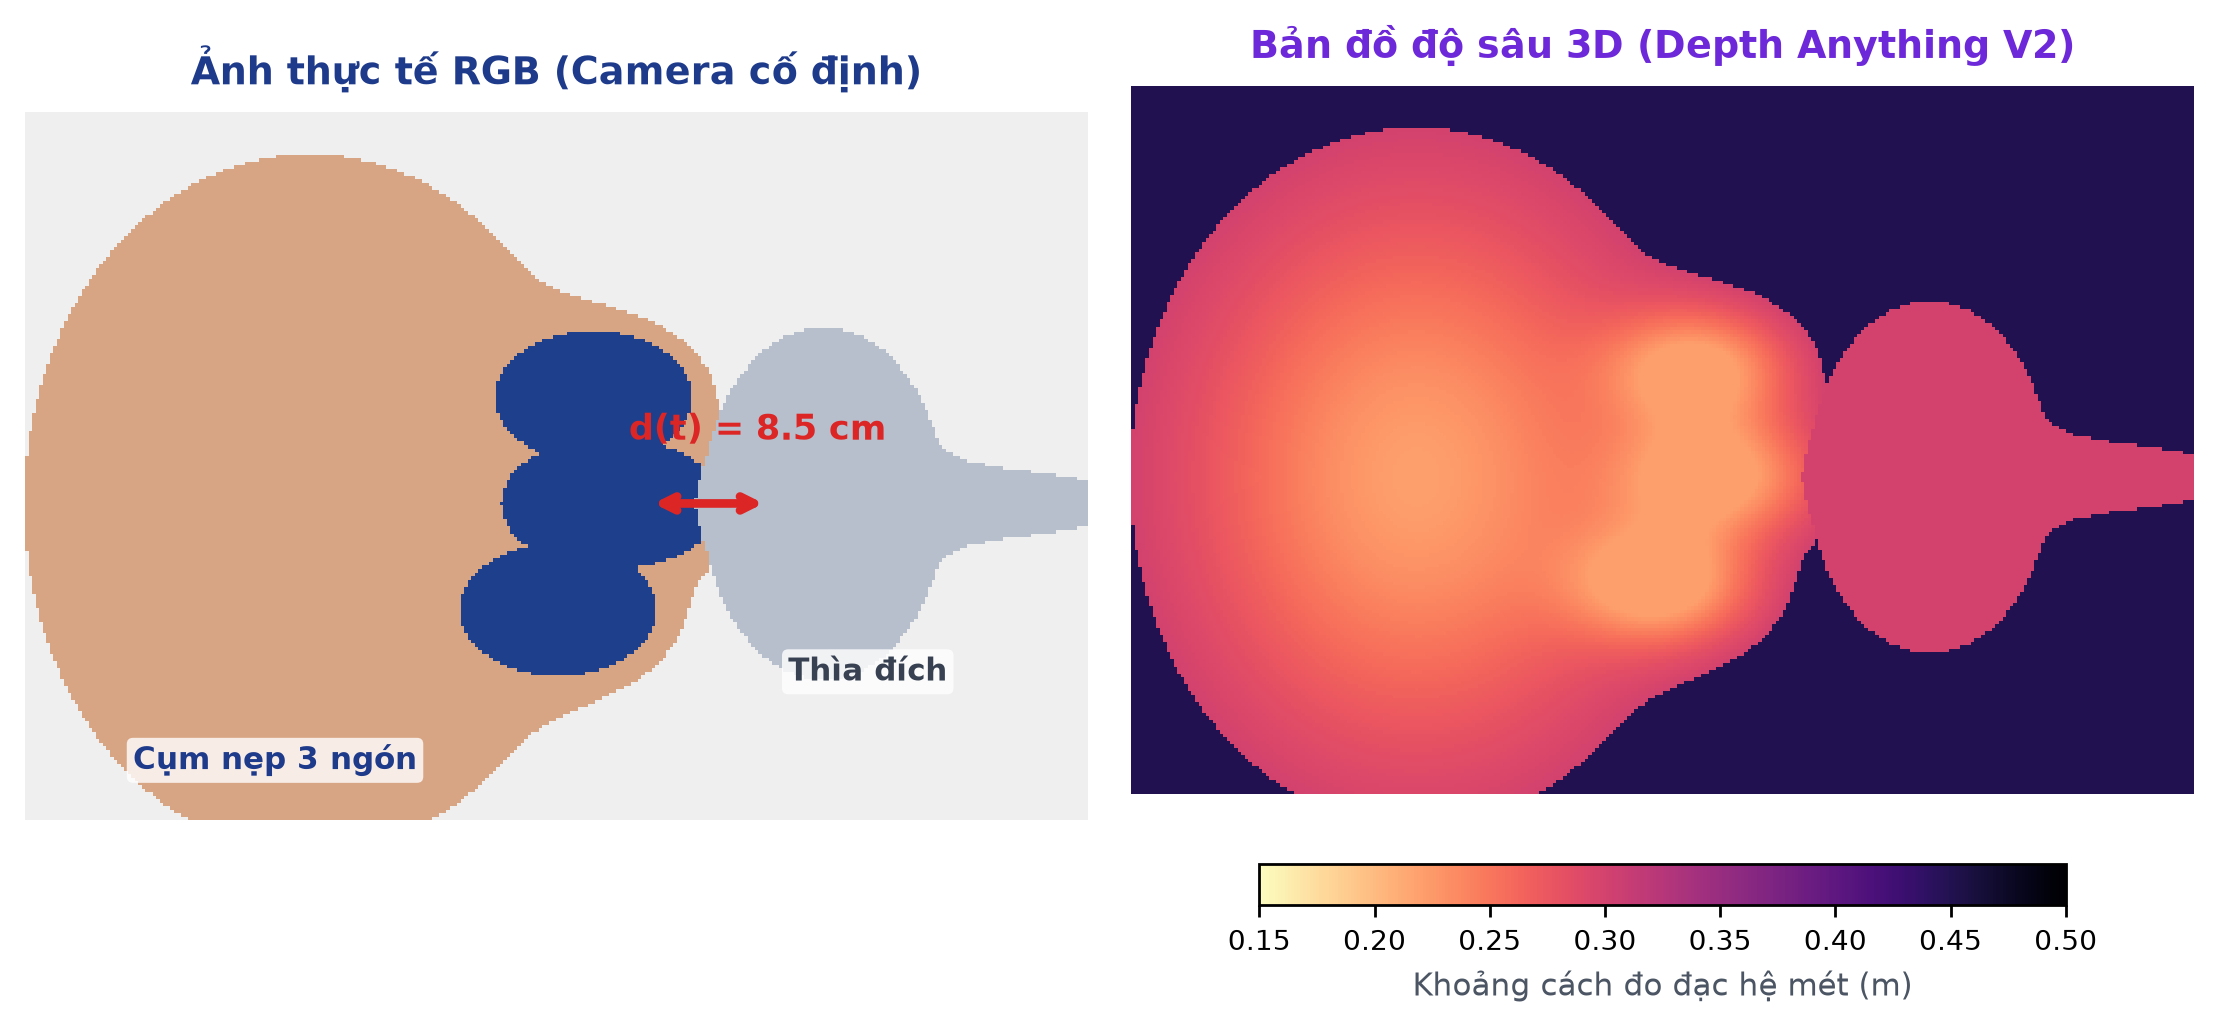
\includegraphics[width=11.5cm, height=2.8cm, keepaspectratio]{assets/depth_anything_scene.png}\\[8pt]
  {\fontsize{16}{20}\selectfont\bfseries Orange Pi 5 Pro + Camera RGB (Depth Anything V2)}\\[4pt]
  {\fontsize{14}{17}\selectfont Ước lượng cự ly 3D $d(t)$ \& Thời gian tới tiếp xúc (TTC) đón trước}
};

% ==================== 2. TẦNG 2: THU THẬP & DSP (ĐẶT PHÍA DƯỚI TẦNG 4 CÁCH 55PT - ZERO COLLISION) ====================
\node[tierCard, text width=9.2cm, below=55pt of tier4] (tier2) {
  {\fontsize{21}{25}\selectfont\bfseries TẦNG 2: THU THẬP \& DSP}\\[3pt]
  {\fontsize{13}{16}\selectfont\color{black!75} (Sensing \& DSP Tier)}\\[10pt]
  
  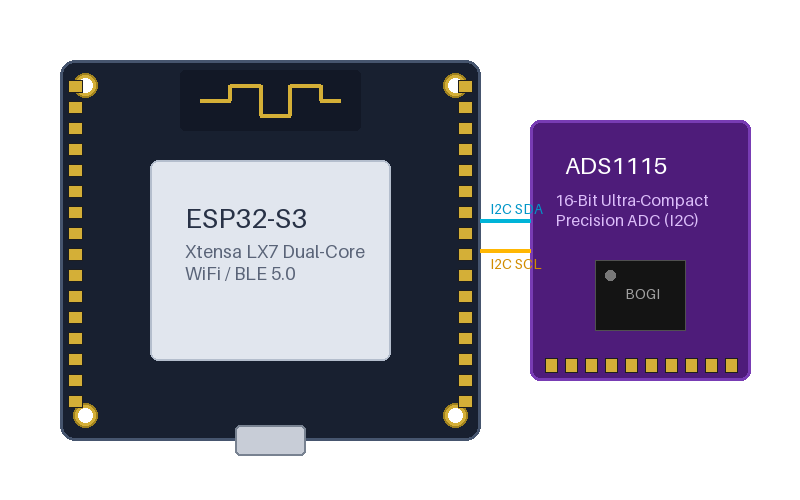
\includegraphics[width=7.5cm, height=3.8cm, keepaspectratio]{assets/controller_ads_board.png}\\[10pt]
  {\fontsize{16}{20}\selectfont\bfseries ESP32-S3 + ADC ADS1115 (16-bit)}\\[4pt]
  {\fontsize{14}{17}\selectfont 2 MUX CD74HC4067 (Thu thập 21 kênh $\ge$15Hz)}\\[12pt]
  
  {\fontsize{16}{20}\selectfont\bfseries Xử lý tín hiệu số (DSP) \& Bộ chỉ số}\\[4pt]
  {\fontsize{14}{17}\selectfont Bám nền khử trôi tĩnh $\bullet$ Tính EI -- GAP -- RAL}\\[4pt]
  {\fontsize{14}{17}\selectfont\bfseries Thuật toán AAN 3 pha trợ lực theo nhu cầu}
};

% ==================== 3. TẦNG 1: TẦNG ĐEO (BÊN TRÁI - DÙNG ẢNH GLOVE HERO SIÊU TO NÉT) ====================
\node[tierCard, text width=9.2cm, left=75pt of tier2.north west, anchor=north east] (tier1) {
  {\fontsize{21}{25}\selectfont\bfseries TẦNG 1: TẦNG ĐEO}\\[3pt]
  {\fontsize{13}{16}\selectfont\color{black!75} (Wearable Physical Tier)}\\[10pt]
  
  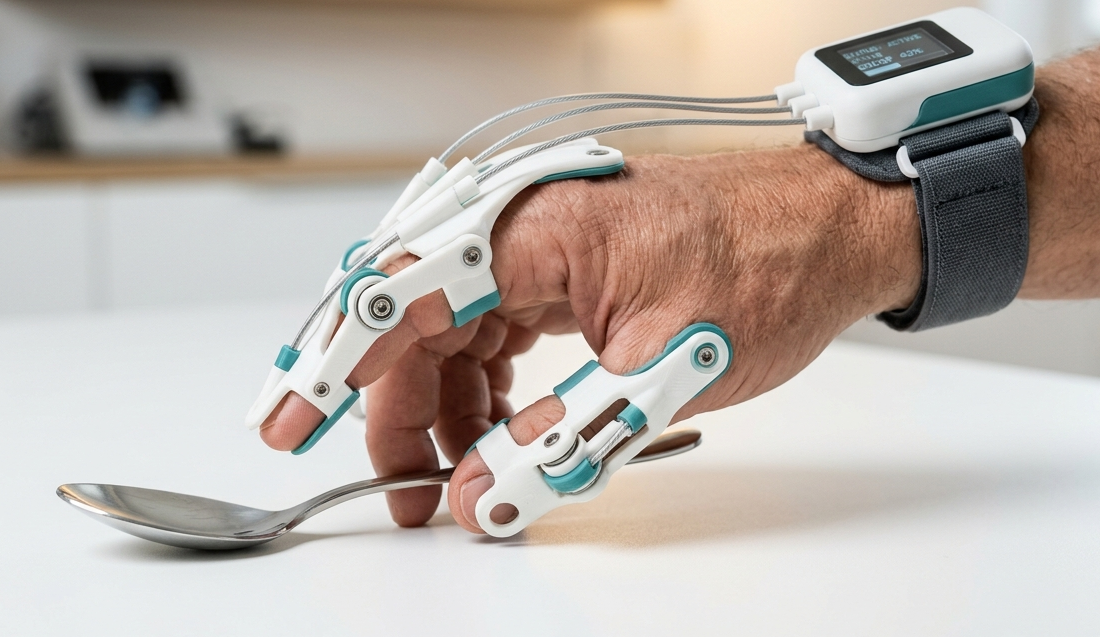
\includegraphics[width=8.2cm, height=4.4cm, keepaspectratio]{assets/real_glove_hero.png}\\[8pt]
  {\fontsize{16}{20}\selectfont\bfseries Khung nẹp 3 ngón in 3D (Cái -- Trỏ -- Giữa)}\\[4pt]
  {\fontsize{14}{17}\selectfont Ngàm xoay 2 bản lề tháo mở độc lập 1 tay}\\[12pt]
  
  {\fontsize{16}{20}\selectfont\bfseries Mạng cảm biến tiếp xúc \& góc uốn}\\[4pt]
  {\fontsize{14}{17}\selectfont 16 Ô Velostat vi sai lòng--mu bàn tay}\\[4pt]
  {\fontsize{14}{17}\selectfont 3 Cảm biến uốn Flex đo góc khớp ngón}
};

% ==================== 4. TẦNG 3: TRỢ LỰC CƠ HỌC (BÊN PHẢI) ====================
\node[tierCard, text width=9.2cm, right=75pt of tier2.north east, anchor=north west] (tier3) {
  {\fontsize{21}{25}\selectfont\bfseries TẦNG 3: TRỢ LỰC}\\[3pt]
  {\fontsize{13}{16}\selectfont\color{black!75} (Actuation Tier)}\\[10pt]
  
  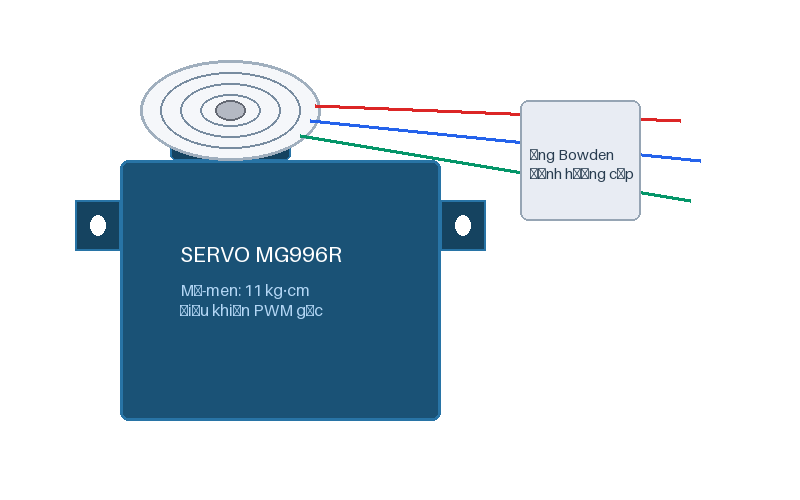
\includegraphics[width=7.5cm, height=3.8cm, keepaspectratio]{assets/servo_spool_assembly.png}\\[10pt]
  {\fontsize{16}{20}\selectfont\bfseries 3 Động cơ Servo MG996R \& Tang cáp}\\[4pt]
  {\fontsize{14}{17}\selectfont Lực kéo chủ động 11 kg$\cdot$cm trên 3 ngón}\\[12pt]
  
  {\fontsize{16}{20}\selectfont\bfseries Cơ cấu truyền động cáp Bowden}\\[4pt]
  {\fontsize{14}{17}\selectfont Cáp Dyneema trợ lực kéo gập ngón chủ động}\\[4pt]
  {\fontsize{14}{17}\selectfont Nẹp đàn hồi hồi vị đẩy mở ngón an toàn}
};

% ==================== MŨI TÊN KẾT NỐI LUỒNG TÍN HIỆU & ĐIỀU KHIỂN ====================

% Tầng 1 -> Tầng 2: Tín hiệu tương tự 21 kênh
\draw[arrowThick] (tier1.east) -- 
  node[tagText, above=4pt] {Tín hiệu 21 kênh} 
  node[tagText, below=4pt] {Lực vi sai \& Góc} 
  (tier2.west);

% Tầng 2 -> Tầng 3: Lệnh điều khiển servo AAN
\draw[arrowThick] (tier2.east) -- 
  node[tagText, above=4pt] {Lệnh servo AAN} 
  node[tagText, below=4pt] {Kéo gập / Nhả duỗi} 
  (tier3.west);

% Tầng 4 -> Tầng 2: Cự ly 3D và TTC đón trước (UART/USB)
\draw[arrowThick] (tier4.south) -- 
  node[tagText, midway] {Khẩu độ \& TTC đón trước (UART)} 
  (tier2.north);

% Tầng 4 -> Tầng 1: Quan sát không gian bài tập
\draw[arrowThick, dashed] (tier4.west) -| 
  node[tagText, pos=0.35, above=4pt] {Quan sát cự ly 3D tay -- thìa} 
  (tier1.north);

% ==================== VÒNG PHẢN HỒI CƠ HỌC (ĐÁY): TẦNG 3 -> TẦNG 1 ====================
\draw[arrowThick] (tier3.south) -- ++(0, -1.5cm) coordinate (p3)
  -- ($(p3) - (20.5cm, 0)$) coordinate (p1)
  node[tagText, midway, below=4pt] {Vòng phản hồi cơ học: Cáp Bowden kéo trợ lực gập ngón / Nhả duỗi mở khẩu độ} 
  -- (tier1.south);

\end{tikzpicture}
\end{document}
